\documentclass[../thesis.tex]{subfiles}

\begin{document}

% \begin{figure}[H]
%     \begin{minipage}{0.45\textwidth}
%         \centering
%         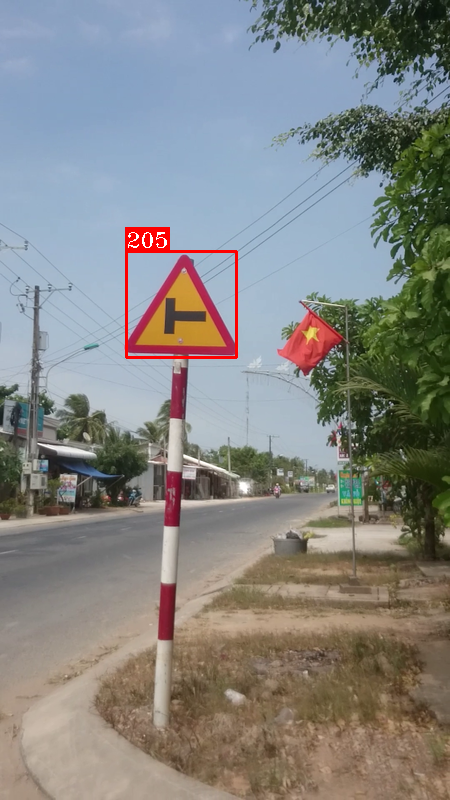
\includegraphics[width=\linewidth]{205_0361.png}
%         \label{Fig:205_0361}
%     \end{minipage}\hfill
%         \begin {minipage}{0.45\textwidth}
%         \centering
%         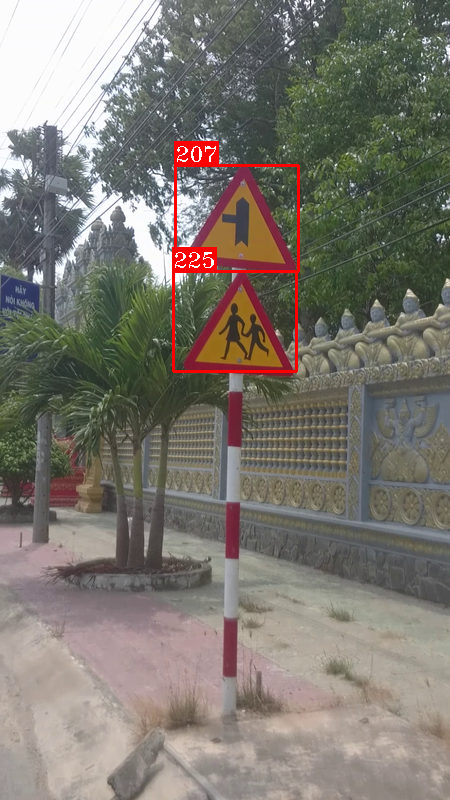
\includegraphics[width=\linewidth]{207_0367.png}
%         \label{Fig:207_0367}
%     \end{minipage}
% \end{figure}

Chúng tôi tiến hành đánh giá mô hình theo 2 kịch bản. Đầu tiên, chúng tôi đánh giá theo cách thông thường, sử dụng tập dữ liệu đánh giá (20\% tập dữ liệu). Sau khi đánh giá theo cách này, chúng tôi nhận thấy mô hình bị hạn chế ở một số điểm, chúng tôi tinh chỉnh tập dữ liệu và đánh giá lại thì mô hình đạt được độ chính xác cao hơn, đồng thời tìm ra nguyên nhân dẫn đến những điểm hạn chế của mô hình. 

Tiêu chí để đánh giá mô hình như sau:

\begin{itemize}[topsep=0pt]
    \item True Positive (TP): Mô hình dự đoán đúng lớp của đối tượng và khung chứa đối tượng được dự đoán bởi mô hình (bounding-box) và khung chứa đối tượng thực sự (ground-truth box) có giá trị IoU lớn hơn 0.5.
    \item False Negative (FN): Đối tượng hiện diện trong ảnh nhưng mô hình không thể nhận ra đối tượng.
    \item False Positive (FP): Mô hình dự đoán đúng lớp của đối tượng nhưng khung chứa đối tượng được dự đoán bởi mô hình và khung chứa đối tượng thực sự có giá trị IoU nhỏ hơn 0.5 hoặc mô hình dự đoán sai lớp của đối tượng.
\end{itemize}

\section{Kịch bản 1: Đánh giá theo cách thông thường}

Kết quả đánh giá mô hình theo kịch bản này được cho trong Bảng \ref{Table:eval_scenario_1}.

\begin{longtable}{| c | l | c | c | c |}
    \hline
    \thead{STT} & \thead{Biển báo} & \thead{True Positive} & \thead{False Negative} & \thead{False Positive}\\
    \hline
    1 & 102 & 16 & 6 & 0\\
    \hline
    2 & 130 & 25 & 39 & 0\\
    \hline 
    3 & 131 & 28 & 26 & 0\\
    \hline
    4 & 201a & 14 & 11 & 10\\
    \hline
    5 & 201b & 31 & 8 & 4\\
    \hline
    6 & 202 & 35 & 4 & 1\\
    \hline
    7 & 203 & 4 & 20 & 1\\
    \hline
    8 & 205 & 63 & 15 & 0\\
    \hline 
    9 & 207 & 171 & 11 & 0\\
    \hline
    10 & 208 & 22 & 7 & 0\\
    \hline
    11 & 209 & 15 & 10 & 0\\
    \hline
    12 & 221 & 16 & 0 & 0\\
    \hline
    13 & 224 & 90 & 10 & 0\\
    \hline
    14 & 225 & 102 & 13 & 0\\
    \hline
    15 & 233 & 21 & 4 & 0\\
    \hline
    16 & 245 & 9 & 3 & 0\\
    \hline
    17 & 302 & 0 & 54 & 0\\
    \hline
    18 & 303 & 15 & 7 & 0\\
    \hline
    19 & 423 & 73 & 17 & 0\\
    \hline
    20 & crowded & 7 & 2 & 1\\
    \hline
    21 & end\_crowded & 0 & 8 & 0\\ 
    \hline
    22 & traffic\_light & 1 & 94 & 0\\
    \hline
    \multicolumn{2}{|c|}{\textbf{Tổng}} & \textbf{758} & \textbf{369} & \textbf{17}\\
    \hline
    \caption{Kết quả đánh giá mô hình theo kịch bản 1}
    \label{Table:eval_scenario_1}
\end{longtable}

Từ kết quả đánh giá trên, ta có thể tính được các chỉ số của mô hình.

$\text{Precision} = \displaystyle\frac{\text{TP}}{\text{TP} + \text{FP}} = \frac{758}{758 + 17} \approx 0.98$

$\text{Recall} = \displaystyle\frac{\text{TP}}{\text{TP} + \text{FN}} = \frac{758}{758 + 369} \approx 0.67$

$\text{F1} = 2 \times \displaystyle\frac{\text{Precision} \times \text{Recall}}{\text{Precision} + \text{Recall}} = 2 \times \frac{0.98 \times 0.67}{0.98 + 0.67} \approx 0.80$

Qua các kết quả đánh giá, ta có thể phán đoán được nguyên nhân dẫn đến những sai số của mô hình như sau:

\begin{itemize}[topsep=0pt]
    \item Kích thước của đối tượng quá nhỏ so với kích cỡ ảnh.
    \item Một số lớp bị thiếu dữ liệu dẫn tới kết quả nhận dạng kém.
	\item Hạn chế của mô hình rút gọn.
\end{itemize} 

\section{Kịch bản 2: Kiểm tra lại mô hình với tập dữ liệu đã qua tinh chỉnh}
% TODO: Cần giải thích thêm 1 chút về kịch bản này là độ chính xác trong kịch bản này sẽ gần với thực tế hơn chứ ko phải chỉ nhằm tăng độ chính xác của mô hình vì mục tiêu của đề tài là sử dụng trong các camera hành trình nên một biển báo có thể xuất hiện trong nhiểu frame và kích thước sẽ tăng dần khi xe tiến đến gần biển báo. Do đó, nếu ở xa mô hình chưa phát hiện thì khi đến gần sẽ phát hiện được.

Từ những phán đoán được đưa ra ở kịch bản 1, chúng tôi đã tiến hành tinh chỉnh lại tập dữ liệu bằng cách cắt cúp các ảnh chứa các đối tượng nhỏ để cải tiến kích thước của đối tượng so với kích cỡ ảnh. Việc đánh giá theo kịch bản này không nhằm nâng cao độ chính xác của mô hình mà chỉ nhằm kiểm định lại những phán đoán được đưa ra ở kịch bản 1. Mặt khác, trong thực tế, camera sẽ di chuyển từ xa tiến lại gần đối tượng biển báo, việc mô hình không nhận dạng được các biển báo quá nhỏ ở xa nhưng lại nhận dạng được các biển báo khi tiến lại gần hơn là có thể chấp nhận được.

Kết quả đánh giá mô hình theo kịch bản 2 được cho trong Bảng \ref{Table:eval_scenario_2}.

\begin{longtable}{| c | l | c | c | c |}
    \hline
    \thead{STT} & \thead{Biển báo} & \thead{True Positive} & \thead{False Negative} & \thead{False Positive}\\
    \hline
    1 & 102 & 22 & 0 & 0\\
    \hline
    2 & 130 & 61 & 4 & 1\\
    \hline 
    3 & 131 & 54 & 0 & 0\\
    \hline
    4 & 201a & 21 & 0 & 15\\
    \hline
    5 & 201b & 36 & 0 & 9\\
    \hline
    6 & 202 & 41 & 0 & 0\\
    \hline
    7 & 203 & 12 & 1 & 22\\
    \hline
    8 & 205 & 78 & 0 & 1\\
    \hline 
    9 & 207 & 180 & 1 & 1\\
    \hline
    10 & 208 & 29 & 0 & 0\\
    \hline
    11 & 209 & 25 & 0 & 0\\
    \hline
    12 & 221 & 16 & 0 & 0\\
    \hline
    13 & 224 & 99 & 1 & 0\\
    \hline
    14 & 225 & 115 & 0 & 1\\
    \hline
    15 & 233 & 23 & 0 & 1\\
    \hline
    16 & 245 & 12 & 0 & 0\\
    \hline
    17 & 302 & 40 & 14 & 0\\
    \hline
    18 & 303 & 20 & 2 & 1\\
    \hline
    19 & 423 & 90 & 0 & 0\\
    \hline
    20 & crowded & 9 & 0 & 2\\
    \hline
    21 & end\_crowded & 5 & 1 & 4\\
    \hline
    22 & traffic\_light & 1 & 94 & 0\\
    \hline
    \multicolumn{2}{|c|}{\textbf{Tổng}} & \textbf{1005} & \textbf{118} & \textbf{58}\\
    \hline
    \caption{Kết quả đánh giá mô hình theo kịch bản 2}
    \label{Table:eval_scenario_2}
\end{longtable}

$\text{Precision} = \displaystyle\frac{\text{TP}}{\text{TP} + \text{FP}} = \frac{1005}{1005 + 58} \approx 0.95$

$\text{Recall} = \displaystyle\frac{\text{TP}}{\text{TP} + \text{FN}} = \frac{1005}{1005 + 118} \approx 0.89$

$\text{F1} = 2 \times \displaystyle\frac{\text{Precision} \times \text{Recall}}{\text{Precision} + \text{Recall}} = 2 \times \frac{0.95 \times 0.89}{0.95 + 0.89} \approx 0.92$

Từ kết quả đánh giá trên, ta có thể thấy rằng những phán đoán được đưa ra ở kịch bản 1 là hoàn toàn hợp lý. Đa số các trường hợp mô hình không nhận dạng được đối tượng (False Negative) đều được giải quyết thông qua việc cải thiện kích thước của đối tượng so với toàn bức ảnh.

\end{document}